\documentclass[11pt,a4paper]{article}

% shared/macros.tex
% Shared notation for all surface-partition math documents.
% Include with: % shared/macros.tex
% Shared notation for all surface-partition math documents.
% Include with: % shared/macros.tex
% Shared notation for all surface-partition math documents.
% Include with: \input{../shared/macros}

% -------------------------------------------------------------------------
% Packages (include here so each document only needs \input{../shared/macros})
% -------------------------------------------------------------------------
\usepackage{amsmath,amssymb,amsthm}
\usepackage{bm}           % \bm for bold math
\usepackage{mathtools}    % \coloneqq, dcases, etc.
\usepackage{booktabs}     % \toprule etc. in tables
\usepackage{hyperref}
\usepackage{geometry}
\usepackage{microtype}
\usepackage{parskip}
\usepackage{xcolor}
\usepackage{tcolorbox}
\usepackage{enumitem}
\usepackage{float}             % [H] float placement

\geometry{a4paper, margin=2.5cm}

% -------------------------------------------------------------------------
% Theorem-like environments
% -------------------------------------------------------------------------
\theoremstyle{definition}
\newtheorem{defn}{Definition}[section]
\newtheorem{remark}{Remark}[section]

\theoremstyle{plain}
\newtheorem{prop}{Proposition}[section]

% -------------------------------------------------------------------------
% Mesh and geometry
% -------------------------------------------------------------------------
\newcommand{\V}{\mathbf{V}}            % vertex array V[i] in R^dim
\newcommand{\F}{\mathbf{F}}            % face (triangle) array
\newcommand{\vone}[1]{v_{1,#1}}       % first vertex index of VP i
\newcommand{\vtwo}[1]{v_{2,#1}}       % second vertex index of VP i

% -------------------------------------------------------------------------
% Variable points
% -------------------------------------------------------------------------
\newcommand{\lam}{\lambda}             % scalar VP parameter
\newcommand{\Lam}{\boldsymbol{\lambda}}% full parameter vector
\newcommand{\vp}[1]{\mathbf{p}_{#1}}  % 3D position of VP i
\newcommand{\ed}[1]{\mathbf{d}_{#1}}  % edge direction d_i = V[v1_i] - V[v2_i]

% -------------------------------------------------------------------------
% Steiner / triple-point
% -------------------------------------------------------------------------
\newcommand{\Sv}{\mathbf{S}}           % Steiner (Fermat-Torricelli) point
\newcommand{\Ki}{K_{i}}               % projection matrix (I-n_i n_i^T)/r_i
\newcommand{\Mmat}{M}                 % sum of K_i matrices at a triple point

% -------------------------------------------------------------------------
% Normals and unit vectors
% -------------------------------------------------------------------------
\newcommand{\nhat}{\hat{\mathbf{n}}}  % unit normal to a triangle
\newcommand{\Dhat}{\hat{\boldsymbol{\Delta}}}  % unit segment direction

% -------------------------------------------------------------------------
% Operations
% -------------------------------------------------------------------------
\newcommand{\norm}[1]{\left\|#1\right\|}
\newcommand{\abs}[1]{\left|#1\right|}
\newcommand{\ip}[2]{\langle #1,\, #2 \rangle}

% Projection perpendicular to a unit vector \uhat
\newcommand{\Proj}[1]{\bigl(\mathbf{I} - #1 #1^\top\bigr)}

% argmax operator (winner-take-all assignment in Phase 1 documents)
\DeclareMathOperator*{\argmax}{arg\,max}
\DeclareMathOperator*{\argmin}{arg\,min}

% -------------------------------------------------------------------------
% Calculus shorthands
% -------------------------------------------------------------------------
\newcommand{\pd}[2]{\dfrac{\partial #1}{\partial #2}}
\newcommand{\pdd}[3]{\dfrac{\partial^2 #1}{\partial #2\,\partial #3}}
\newcommand{\grad}{\nabla}
\newcommand{\Hess}[1]{\nabla^2 #1}

% -------------------------------------------------------------------------
% Optimization problem objects
% -------------------------------------------------------------------------
\newcommand{\Preg}{P_{\mathrm{reg}}}  % regular perimeter
\newcommand{\Pst}{P_{\mathrm{st}}}   % Steiner perimeter
\newcommand{\Areg}{A^{\mathrm{reg}}} % regular cell area
\newcommand{\Ast}{A^{\mathrm{st}}}   % Steiner area contribution
\newcommand{\Atgt}{\bar{A}}           % target area per cell
\newcommand{\Lagr}{\mathcal{L}}       % Lagrangian
\newcommand{\objfac}{\sigma}          % IPOPT objective scaling factor

% -------------------------------------------------------------------------
% Code cross-references (for "In the code..." callouts)
% -------------------------------------------------------------------------
\newcommand{\code}[1]{\texttt{#1}}
\newcommand{\codefile}[1]{\texttt{\small #1}}

% -------------------------------------------------------------------------
% Threshold dynamics / approach B (10-mbo-auction-dynamics)
% -------------------------------------------------------------------------
\newcommand{\Dlump}{D}                 % lumped mass matrix diag(v)
\newcommand{\Atau}{A_\tau}             % discrete diffusion operator (M + tau K)^{-1} M
\newcommand{\Etau}{E_\tau}             % heat-content (threshold-dynamics) energy
\newcommand{\Rcell}{R_{\mathrm{cell}}} % radius of the equal-area disc sqrt(Abar/pi)
\newcommand{\hmean}{h_{\mathrm{mean}}} % mean edge length
\newcommand{\hmax}{h_{\mathrm{max}}}   % max edge length
\newcommand{\Gt}{G_t}                  % heat kernel at time t
\newcommand{\Ktau}{K^{\mathrm{res}}_\tau} % resolvent (backward-Euler) kernel


% -------------------------------------------------------------------------
% Packages (include here so each document only needs % shared/macros.tex
% Shared notation for all surface-partition math documents.
% Include with: \input{../shared/macros}

% -------------------------------------------------------------------------
% Packages (include here so each document only needs \input{../shared/macros})
% -------------------------------------------------------------------------
\usepackage{amsmath,amssymb,amsthm}
\usepackage{bm}           % \bm for bold math
\usepackage{mathtools}    % \coloneqq, dcases, etc.
\usepackage{booktabs}     % \toprule etc. in tables
\usepackage{hyperref}
\usepackage{geometry}
\usepackage{microtype}
\usepackage{parskip}
\usepackage{xcolor}
\usepackage{tcolorbox}
\usepackage{enumitem}
\usepackage{float}             % [H] float placement

\geometry{a4paper, margin=2.5cm}

% -------------------------------------------------------------------------
% Theorem-like environments
% -------------------------------------------------------------------------
\theoremstyle{definition}
\newtheorem{defn}{Definition}[section]
\newtheorem{remark}{Remark}[section]

\theoremstyle{plain}
\newtheorem{prop}{Proposition}[section]

% -------------------------------------------------------------------------
% Mesh and geometry
% -------------------------------------------------------------------------
\newcommand{\V}{\mathbf{V}}            % vertex array V[i] in R^dim
\newcommand{\F}{\mathbf{F}}            % face (triangle) array
\newcommand{\vone}[1]{v_{1,#1}}       % first vertex index of VP i
\newcommand{\vtwo}[1]{v_{2,#1}}       % second vertex index of VP i

% -------------------------------------------------------------------------
% Variable points
% -------------------------------------------------------------------------
\newcommand{\lam}{\lambda}             % scalar VP parameter
\newcommand{\Lam}{\boldsymbol{\lambda}}% full parameter vector
\newcommand{\vp}[1]{\mathbf{p}_{#1}}  % 3D position of VP i
\newcommand{\ed}[1]{\mathbf{d}_{#1}}  % edge direction d_i = V[v1_i] - V[v2_i]

% -------------------------------------------------------------------------
% Steiner / triple-point
% -------------------------------------------------------------------------
\newcommand{\Sv}{\mathbf{S}}           % Steiner (Fermat-Torricelli) point
\newcommand{\Ki}{K_{i}}               % projection matrix (I-n_i n_i^T)/r_i
\newcommand{\Mmat}{M}                 % sum of K_i matrices at a triple point

% -------------------------------------------------------------------------
% Normals and unit vectors
% -------------------------------------------------------------------------
\newcommand{\nhat}{\hat{\mathbf{n}}}  % unit normal to a triangle
\newcommand{\Dhat}{\hat{\boldsymbol{\Delta}}}  % unit segment direction

% -------------------------------------------------------------------------
% Operations
% -------------------------------------------------------------------------
\newcommand{\norm}[1]{\left\|#1\right\|}
\newcommand{\abs}[1]{\left|#1\right|}
\newcommand{\ip}[2]{\langle #1,\, #2 \rangle}

% Projection perpendicular to a unit vector \uhat
\newcommand{\Proj}[1]{\bigl(\mathbf{I} - #1 #1^\top\bigr)}

% argmax operator (winner-take-all assignment in Phase 1 documents)
\DeclareMathOperator*{\argmax}{arg\,max}
\DeclareMathOperator*{\argmin}{arg\,min}

% -------------------------------------------------------------------------
% Calculus shorthands
% -------------------------------------------------------------------------
\newcommand{\pd}[2]{\dfrac{\partial #1}{\partial #2}}
\newcommand{\pdd}[3]{\dfrac{\partial^2 #1}{\partial #2\,\partial #3}}
\newcommand{\grad}{\nabla}
\newcommand{\Hess}[1]{\nabla^2 #1}

% -------------------------------------------------------------------------
% Optimization problem objects
% -------------------------------------------------------------------------
\newcommand{\Preg}{P_{\mathrm{reg}}}  % regular perimeter
\newcommand{\Pst}{P_{\mathrm{st}}}   % Steiner perimeter
\newcommand{\Areg}{A^{\mathrm{reg}}} % regular cell area
\newcommand{\Ast}{A^{\mathrm{st}}}   % Steiner area contribution
\newcommand{\Atgt}{\bar{A}}           % target area per cell
\newcommand{\Lagr}{\mathcal{L}}       % Lagrangian
\newcommand{\objfac}{\sigma}          % IPOPT objective scaling factor

% -------------------------------------------------------------------------
% Code cross-references (for "In the code..." callouts)
% -------------------------------------------------------------------------
\newcommand{\code}[1]{\texttt{#1}}
\newcommand{\codefile}[1]{\texttt{\small #1}}

% -------------------------------------------------------------------------
% Threshold dynamics / approach B (10-mbo-auction-dynamics)
% -------------------------------------------------------------------------
\newcommand{\Dlump}{D}                 % lumped mass matrix diag(v)
\newcommand{\Atau}{A_\tau}             % discrete diffusion operator (M + tau K)^{-1} M
\newcommand{\Etau}{E_\tau}             % heat-content (threshold-dynamics) energy
\newcommand{\Rcell}{R_{\mathrm{cell}}} % radius of the equal-area disc sqrt(Abar/pi)
\newcommand{\hmean}{h_{\mathrm{mean}}} % mean edge length
\newcommand{\hmax}{h_{\mathrm{max}}}   % max edge length
\newcommand{\Gt}{G_t}                  % heat kernel at time t
\newcommand{\Ktau}{K^{\mathrm{res}}_\tau} % resolvent (backward-Euler) kernel
)
% -------------------------------------------------------------------------
\usepackage{amsmath,amssymb,amsthm}
\usepackage{bm}           % \bm for bold math
\usepackage{mathtools}    % \coloneqq, dcases, etc.
\usepackage{booktabs}     % \toprule etc. in tables
\usepackage{hyperref}
\usepackage{geometry}
\usepackage{microtype}
\usepackage{parskip}
\usepackage{xcolor}
\usepackage{tcolorbox}
\usepackage{enumitem}
\usepackage{float}             % [H] float placement

\geometry{a4paper, margin=2.5cm}

% -------------------------------------------------------------------------
% Theorem-like environments
% -------------------------------------------------------------------------
\theoremstyle{definition}
\newtheorem{defn}{Definition}[section]
\newtheorem{remark}{Remark}[section]

\theoremstyle{plain}
\newtheorem{prop}{Proposition}[section]

% -------------------------------------------------------------------------
% Mesh and geometry
% -------------------------------------------------------------------------
\newcommand{\V}{\mathbf{V}}            % vertex array V[i] in R^dim
\newcommand{\F}{\mathbf{F}}            % face (triangle) array
\newcommand{\vone}[1]{v_{1,#1}}       % first vertex index of VP i
\newcommand{\vtwo}[1]{v_{2,#1}}       % second vertex index of VP i

% -------------------------------------------------------------------------
% Variable points
% -------------------------------------------------------------------------
\newcommand{\lam}{\lambda}             % scalar VP parameter
\newcommand{\Lam}{\boldsymbol{\lambda}}% full parameter vector
\newcommand{\vp}[1]{\mathbf{p}_{#1}}  % 3D position of VP i
\newcommand{\ed}[1]{\mathbf{d}_{#1}}  % edge direction d_i = V[v1_i] - V[v2_i]

% -------------------------------------------------------------------------
% Steiner / triple-point
% -------------------------------------------------------------------------
\newcommand{\Sv}{\mathbf{S}}           % Steiner (Fermat-Torricelli) point
\newcommand{\Ki}{K_{i}}               % projection matrix (I-n_i n_i^T)/r_i
\newcommand{\Mmat}{M}                 % sum of K_i matrices at a triple point

% -------------------------------------------------------------------------
% Normals and unit vectors
% -------------------------------------------------------------------------
\newcommand{\nhat}{\hat{\mathbf{n}}}  % unit normal to a triangle
\newcommand{\Dhat}{\hat{\boldsymbol{\Delta}}}  % unit segment direction

% -------------------------------------------------------------------------
% Operations
% -------------------------------------------------------------------------
\newcommand{\norm}[1]{\left\|#1\right\|}
\newcommand{\abs}[1]{\left|#1\right|}
\newcommand{\ip}[2]{\langle #1,\, #2 \rangle}

% Projection perpendicular to a unit vector \uhat
\newcommand{\Proj}[1]{\bigl(\mathbf{I} - #1 #1^\top\bigr)}

% argmax operator (winner-take-all assignment in Phase 1 documents)
\DeclareMathOperator*{\argmax}{arg\,max}
\DeclareMathOperator*{\argmin}{arg\,min}

% -------------------------------------------------------------------------
% Calculus shorthands
% -------------------------------------------------------------------------
\newcommand{\pd}[2]{\dfrac{\partial #1}{\partial #2}}
\newcommand{\pdd}[3]{\dfrac{\partial^2 #1}{\partial #2\,\partial #3}}
\newcommand{\grad}{\nabla}
\newcommand{\Hess}[1]{\nabla^2 #1}

% -------------------------------------------------------------------------
% Optimization problem objects
% -------------------------------------------------------------------------
\newcommand{\Preg}{P_{\mathrm{reg}}}  % regular perimeter
\newcommand{\Pst}{P_{\mathrm{st}}}   % Steiner perimeter
\newcommand{\Areg}{A^{\mathrm{reg}}} % regular cell area
\newcommand{\Ast}{A^{\mathrm{st}}}   % Steiner area contribution
\newcommand{\Atgt}{\bar{A}}           % target area per cell
\newcommand{\Lagr}{\mathcal{L}}       % Lagrangian
\newcommand{\objfac}{\sigma}          % IPOPT objective scaling factor

% -------------------------------------------------------------------------
% Code cross-references (for "In the code..." callouts)
% -------------------------------------------------------------------------
\newcommand{\code}[1]{\texttt{#1}}
\newcommand{\codefile}[1]{\texttt{\small #1}}

% -------------------------------------------------------------------------
% Threshold dynamics / approach B (10-mbo-auction-dynamics)
% -------------------------------------------------------------------------
\newcommand{\Dlump}{D}                 % lumped mass matrix diag(v)
\newcommand{\Atau}{A_\tau}             % discrete diffusion operator (M + tau K)^{-1} M
\newcommand{\Etau}{E_\tau}             % heat-content (threshold-dynamics) energy
\newcommand{\Rcell}{R_{\mathrm{cell}}} % radius of the equal-area disc sqrt(Abar/pi)
\newcommand{\hmean}{h_{\mathrm{mean}}} % mean edge length
\newcommand{\hmax}{h_{\mathrm{max}}}   % max edge length
\newcommand{\Gt}{G_t}                  % heat kernel at time t
\newcommand{\Ktau}{K^{\mathrm{res}}_\tau} % resolvent (backward-Euler) kernel


% -------------------------------------------------------------------------
% Packages (include here so each document only needs % shared/macros.tex
% Shared notation for all surface-partition math documents.
% Include with: % shared/macros.tex
% Shared notation for all surface-partition math documents.
% Include with: \input{../shared/macros}

% -------------------------------------------------------------------------
% Packages (include here so each document only needs \input{../shared/macros})
% -------------------------------------------------------------------------
\usepackage{amsmath,amssymb,amsthm}
\usepackage{bm}           % \bm for bold math
\usepackage{mathtools}    % \coloneqq, dcases, etc.
\usepackage{booktabs}     % \toprule etc. in tables
\usepackage{hyperref}
\usepackage{geometry}
\usepackage{microtype}
\usepackage{parskip}
\usepackage{xcolor}
\usepackage{tcolorbox}
\usepackage{enumitem}
\usepackage{float}             % [H] float placement

\geometry{a4paper, margin=2.5cm}

% -------------------------------------------------------------------------
% Theorem-like environments
% -------------------------------------------------------------------------
\theoremstyle{definition}
\newtheorem{defn}{Definition}[section]
\newtheorem{remark}{Remark}[section]

\theoremstyle{plain}
\newtheorem{prop}{Proposition}[section]

% -------------------------------------------------------------------------
% Mesh and geometry
% -------------------------------------------------------------------------
\newcommand{\V}{\mathbf{V}}            % vertex array V[i] in R^dim
\newcommand{\F}{\mathbf{F}}            % face (triangle) array
\newcommand{\vone}[1]{v_{1,#1}}       % first vertex index of VP i
\newcommand{\vtwo}[1]{v_{2,#1}}       % second vertex index of VP i

% -------------------------------------------------------------------------
% Variable points
% -------------------------------------------------------------------------
\newcommand{\lam}{\lambda}             % scalar VP parameter
\newcommand{\Lam}{\boldsymbol{\lambda}}% full parameter vector
\newcommand{\vp}[1]{\mathbf{p}_{#1}}  % 3D position of VP i
\newcommand{\ed}[1]{\mathbf{d}_{#1}}  % edge direction d_i = V[v1_i] - V[v2_i]

% -------------------------------------------------------------------------
% Steiner / triple-point
% -------------------------------------------------------------------------
\newcommand{\Sv}{\mathbf{S}}           % Steiner (Fermat-Torricelli) point
\newcommand{\Ki}{K_{i}}               % projection matrix (I-n_i n_i^T)/r_i
\newcommand{\Mmat}{M}                 % sum of K_i matrices at a triple point

% -------------------------------------------------------------------------
% Normals and unit vectors
% -------------------------------------------------------------------------
\newcommand{\nhat}{\hat{\mathbf{n}}}  % unit normal to a triangle
\newcommand{\Dhat}{\hat{\boldsymbol{\Delta}}}  % unit segment direction

% -------------------------------------------------------------------------
% Operations
% -------------------------------------------------------------------------
\newcommand{\norm}[1]{\left\|#1\right\|}
\newcommand{\abs}[1]{\left|#1\right|}
\newcommand{\ip}[2]{\langle #1,\, #2 \rangle}

% Projection perpendicular to a unit vector \uhat
\newcommand{\Proj}[1]{\bigl(\mathbf{I} - #1 #1^\top\bigr)}

% argmax operator (winner-take-all assignment in Phase 1 documents)
\DeclareMathOperator*{\argmax}{arg\,max}
\DeclareMathOperator*{\argmin}{arg\,min}

% -------------------------------------------------------------------------
% Calculus shorthands
% -------------------------------------------------------------------------
\newcommand{\pd}[2]{\dfrac{\partial #1}{\partial #2}}
\newcommand{\pdd}[3]{\dfrac{\partial^2 #1}{\partial #2\,\partial #3}}
\newcommand{\grad}{\nabla}
\newcommand{\Hess}[1]{\nabla^2 #1}

% -------------------------------------------------------------------------
% Optimization problem objects
% -------------------------------------------------------------------------
\newcommand{\Preg}{P_{\mathrm{reg}}}  % regular perimeter
\newcommand{\Pst}{P_{\mathrm{st}}}   % Steiner perimeter
\newcommand{\Areg}{A^{\mathrm{reg}}} % regular cell area
\newcommand{\Ast}{A^{\mathrm{st}}}   % Steiner area contribution
\newcommand{\Atgt}{\bar{A}}           % target area per cell
\newcommand{\Lagr}{\mathcal{L}}       % Lagrangian
\newcommand{\objfac}{\sigma}          % IPOPT objective scaling factor

% -------------------------------------------------------------------------
% Code cross-references (for "In the code..." callouts)
% -------------------------------------------------------------------------
\newcommand{\code}[1]{\texttt{#1}}
\newcommand{\codefile}[1]{\texttt{\small #1}}

% -------------------------------------------------------------------------
% Threshold dynamics / approach B (10-mbo-auction-dynamics)
% -------------------------------------------------------------------------
\newcommand{\Dlump}{D}                 % lumped mass matrix diag(v)
\newcommand{\Atau}{A_\tau}             % discrete diffusion operator (M + tau K)^{-1} M
\newcommand{\Etau}{E_\tau}             % heat-content (threshold-dynamics) energy
\newcommand{\Rcell}{R_{\mathrm{cell}}} % radius of the equal-area disc sqrt(Abar/pi)
\newcommand{\hmean}{h_{\mathrm{mean}}} % mean edge length
\newcommand{\hmax}{h_{\mathrm{max}}}   % max edge length
\newcommand{\Gt}{G_t}                  % heat kernel at time t
\newcommand{\Ktau}{K^{\mathrm{res}}_\tau} % resolvent (backward-Euler) kernel


% -------------------------------------------------------------------------
% Packages (include here so each document only needs % shared/macros.tex
% Shared notation for all surface-partition math documents.
% Include with: \input{../shared/macros}

% -------------------------------------------------------------------------
% Packages (include here so each document only needs \input{../shared/macros})
% -------------------------------------------------------------------------
\usepackage{amsmath,amssymb,amsthm}
\usepackage{bm}           % \bm for bold math
\usepackage{mathtools}    % \coloneqq, dcases, etc.
\usepackage{booktabs}     % \toprule etc. in tables
\usepackage{hyperref}
\usepackage{geometry}
\usepackage{microtype}
\usepackage{parskip}
\usepackage{xcolor}
\usepackage{tcolorbox}
\usepackage{enumitem}
\usepackage{float}             % [H] float placement

\geometry{a4paper, margin=2.5cm}

% -------------------------------------------------------------------------
% Theorem-like environments
% -------------------------------------------------------------------------
\theoremstyle{definition}
\newtheorem{defn}{Definition}[section]
\newtheorem{remark}{Remark}[section]

\theoremstyle{plain}
\newtheorem{prop}{Proposition}[section]

% -------------------------------------------------------------------------
% Mesh and geometry
% -------------------------------------------------------------------------
\newcommand{\V}{\mathbf{V}}            % vertex array V[i] in R^dim
\newcommand{\F}{\mathbf{F}}            % face (triangle) array
\newcommand{\vone}[1]{v_{1,#1}}       % first vertex index of VP i
\newcommand{\vtwo}[1]{v_{2,#1}}       % second vertex index of VP i

% -------------------------------------------------------------------------
% Variable points
% -------------------------------------------------------------------------
\newcommand{\lam}{\lambda}             % scalar VP parameter
\newcommand{\Lam}{\boldsymbol{\lambda}}% full parameter vector
\newcommand{\vp}[1]{\mathbf{p}_{#1}}  % 3D position of VP i
\newcommand{\ed}[1]{\mathbf{d}_{#1}}  % edge direction d_i = V[v1_i] - V[v2_i]

% -------------------------------------------------------------------------
% Steiner / triple-point
% -------------------------------------------------------------------------
\newcommand{\Sv}{\mathbf{S}}           % Steiner (Fermat-Torricelli) point
\newcommand{\Ki}{K_{i}}               % projection matrix (I-n_i n_i^T)/r_i
\newcommand{\Mmat}{M}                 % sum of K_i matrices at a triple point

% -------------------------------------------------------------------------
% Normals and unit vectors
% -------------------------------------------------------------------------
\newcommand{\nhat}{\hat{\mathbf{n}}}  % unit normal to a triangle
\newcommand{\Dhat}{\hat{\boldsymbol{\Delta}}}  % unit segment direction

% -------------------------------------------------------------------------
% Operations
% -------------------------------------------------------------------------
\newcommand{\norm}[1]{\left\|#1\right\|}
\newcommand{\abs}[1]{\left|#1\right|}
\newcommand{\ip}[2]{\langle #1,\, #2 \rangle}

% Projection perpendicular to a unit vector \uhat
\newcommand{\Proj}[1]{\bigl(\mathbf{I} - #1 #1^\top\bigr)}

% argmax operator (winner-take-all assignment in Phase 1 documents)
\DeclareMathOperator*{\argmax}{arg\,max}
\DeclareMathOperator*{\argmin}{arg\,min}

% -------------------------------------------------------------------------
% Calculus shorthands
% -------------------------------------------------------------------------
\newcommand{\pd}[2]{\dfrac{\partial #1}{\partial #2}}
\newcommand{\pdd}[3]{\dfrac{\partial^2 #1}{\partial #2\,\partial #3}}
\newcommand{\grad}{\nabla}
\newcommand{\Hess}[1]{\nabla^2 #1}

% -------------------------------------------------------------------------
% Optimization problem objects
% -------------------------------------------------------------------------
\newcommand{\Preg}{P_{\mathrm{reg}}}  % regular perimeter
\newcommand{\Pst}{P_{\mathrm{st}}}   % Steiner perimeter
\newcommand{\Areg}{A^{\mathrm{reg}}} % regular cell area
\newcommand{\Ast}{A^{\mathrm{st}}}   % Steiner area contribution
\newcommand{\Atgt}{\bar{A}}           % target area per cell
\newcommand{\Lagr}{\mathcal{L}}       % Lagrangian
\newcommand{\objfac}{\sigma}          % IPOPT objective scaling factor

% -------------------------------------------------------------------------
% Code cross-references (for "In the code..." callouts)
% -------------------------------------------------------------------------
\newcommand{\code}[1]{\texttt{#1}}
\newcommand{\codefile}[1]{\texttt{\small #1}}

% -------------------------------------------------------------------------
% Threshold dynamics / approach B (10-mbo-auction-dynamics)
% -------------------------------------------------------------------------
\newcommand{\Dlump}{D}                 % lumped mass matrix diag(v)
\newcommand{\Atau}{A_\tau}             % discrete diffusion operator (M + tau K)^{-1} M
\newcommand{\Etau}{E_\tau}             % heat-content (threshold-dynamics) energy
\newcommand{\Rcell}{R_{\mathrm{cell}}} % radius of the equal-area disc sqrt(Abar/pi)
\newcommand{\hmean}{h_{\mathrm{mean}}} % mean edge length
\newcommand{\hmax}{h_{\mathrm{max}}}   % max edge length
\newcommand{\Gt}{G_t}                  % heat kernel at time t
\newcommand{\Ktau}{K^{\mathrm{res}}_\tau} % resolvent (backward-Euler) kernel
)
% -------------------------------------------------------------------------
\usepackage{amsmath,amssymb,amsthm}
\usepackage{bm}           % \bm for bold math
\usepackage{mathtools}    % \coloneqq, dcases, etc.
\usepackage{booktabs}     % \toprule etc. in tables
\usepackage{hyperref}
\usepackage{geometry}
\usepackage{microtype}
\usepackage{parskip}
\usepackage{xcolor}
\usepackage{tcolorbox}
\usepackage{enumitem}
\usepackage{float}             % [H] float placement

\geometry{a4paper, margin=2.5cm}

% -------------------------------------------------------------------------
% Theorem-like environments
% -------------------------------------------------------------------------
\theoremstyle{definition}
\newtheorem{defn}{Definition}[section]
\newtheorem{remark}{Remark}[section]

\theoremstyle{plain}
\newtheorem{prop}{Proposition}[section]

% -------------------------------------------------------------------------
% Mesh and geometry
% -------------------------------------------------------------------------
\newcommand{\V}{\mathbf{V}}            % vertex array V[i] in R^dim
\newcommand{\F}{\mathbf{F}}            % face (triangle) array
\newcommand{\vone}[1]{v_{1,#1}}       % first vertex index of VP i
\newcommand{\vtwo}[1]{v_{2,#1}}       % second vertex index of VP i

% -------------------------------------------------------------------------
% Variable points
% -------------------------------------------------------------------------
\newcommand{\lam}{\lambda}             % scalar VP parameter
\newcommand{\Lam}{\boldsymbol{\lambda}}% full parameter vector
\newcommand{\vp}[1]{\mathbf{p}_{#1}}  % 3D position of VP i
\newcommand{\ed}[1]{\mathbf{d}_{#1}}  % edge direction d_i = V[v1_i] - V[v2_i]

% -------------------------------------------------------------------------
% Steiner / triple-point
% -------------------------------------------------------------------------
\newcommand{\Sv}{\mathbf{S}}           % Steiner (Fermat-Torricelli) point
\newcommand{\Ki}{K_{i}}               % projection matrix (I-n_i n_i^T)/r_i
\newcommand{\Mmat}{M}                 % sum of K_i matrices at a triple point

% -------------------------------------------------------------------------
% Normals and unit vectors
% -------------------------------------------------------------------------
\newcommand{\nhat}{\hat{\mathbf{n}}}  % unit normal to a triangle
\newcommand{\Dhat}{\hat{\boldsymbol{\Delta}}}  % unit segment direction

% -------------------------------------------------------------------------
% Operations
% -------------------------------------------------------------------------
\newcommand{\norm}[1]{\left\|#1\right\|}
\newcommand{\abs}[1]{\left|#1\right|}
\newcommand{\ip}[2]{\langle #1,\, #2 \rangle}

% Projection perpendicular to a unit vector \uhat
\newcommand{\Proj}[1]{\bigl(\mathbf{I} - #1 #1^\top\bigr)}

% argmax operator (winner-take-all assignment in Phase 1 documents)
\DeclareMathOperator*{\argmax}{arg\,max}
\DeclareMathOperator*{\argmin}{arg\,min}

% -------------------------------------------------------------------------
% Calculus shorthands
% -------------------------------------------------------------------------
\newcommand{\pd}[2]{\dfrac{\partial #1}{\partial #2}}
\newcommand{\pdd}[3]{\dfrac{\partial^2 #1}{\partial #2\,\partial #3}}
\newcommand{\grad}{\nabla}
\newcommand{\Hess}[1]{\nabla^2 #1}

% -------------------------------------------------------------------------
% Optimization problem objects
% -------------------------------------------------------------------------
\newcommand{\Preg}{P_{\mathrm{reg}}}  % regular perimeter
\newcommand{\Pst}{P_{\mathrm{st}}}   % Steiner perimeter
\newcommand{\Areg}{A^{\mathrm{reg}}} % regular cell area
\newcommand{\Ast}{A^{\mathrm{st}}}   % Steiner area contribution
\newcommand{\Atgt}{\bar{A}}           % target area per cell
\newcommand{\Lagr}{\mathcal{L}}       % Lagrangian
\newcommand{\objfac}{\sigma}          % IPOPT objective scaling factor

% -------------------------------------------------------------------------
% Code cross-references (for "In the code..." callouts)
% -------------------------------------------------------------------------
\newcommand{\code}[1]{\texttt{#1}}
\newcommand{\codefile}[1]{\texttt{\small #1}}

% -------------------------------------------------------------------------
% Threshold dynamics / approach B (10-mbo-auction-dynamics)
% -------------------------------------------------------------------------
\newcommand{\Dlump}{D}                 % lumped mass matrix diag(v)
\newcommand{\Atau}{A_\tau}             % discrete diffusion operator (M + tau K)^{-1} M
\newcommand{\Etau}{E_\tau}             % heat-content (threshold-dynamics) energy
\newcommand{\Rcell}{R_{\mathrm{cell}}} % radius of the equal-area disc sqrt(Abar/pi)
\newcommand{\hmean}{h_{\mathrm{mean}}} % mean edge length
\newcommand{\hmax}{h_{\mathrm{max}}}   % max edge length
\newcommand{\Gt}{G_t}                  % heat kernel at time t
\newcommand{\Ktau}{K^{\mathrm{res}}_\tau} % resolvent (backward-Euler) kernel
)
% -------------------------------------------------------------------------
\usepackage{amsmath,amssymb,amsthm}
\usepackage{bm}           % \bm for bold math
\usepackage{mathtools}    % \coloneqq, dcases, etc.
\usepackage{booktabs}     % \toprule etc. in tables
\usepackage{hyperref}
\usepackage{geometry}
\usepackage{microtype}
\usepackage{parskip}
\usepackage{xcolor}
\usepackage{tcolorbox}
\usepackage{enumitem}
\usepackage{float}             % [H] float placement

\geometry{a4paper, margin=2.5cm}

% -------------------------------------------------------------------------
% Theorem-like environments
% -------------------------------------------------------------------------
\theoremstyle{definition}
\newtheorem{defn}{Definition}[section]
\newtheorem{remark}{Remark}[section]

\theoremstyle{plain}
\newtheorem{prop}{Proposition}[section]

% -------------------------------------------------------------------------
% Mesh and geometry
% -------------------------------------------------------------------------
\newcommand{\V}{\mathbf{V}}            % vertex array V[i] in R^dim
\newcommand{\F}{\mathbf{F}}            % face (triangle) array
\newcommand{\vone}[1]{v_{1,#1}}       % first vertex index of VP i
\newcommand{\vtwo}[1]{v_{2,#1}}       % second vertex index of VP i

% -------------------------------------------------------------------------
% Variable points
% -------------------------------------------------------------------------
\newcommand{\lam}{\lambda}             % scalar VP parameter
\newcommand{\Lam}{\boldsymbol{\lambda}}% full parameter vector
\newcommand{\vp}[1]{\mathbf{p}_{#1}}  % 3D position of VP i
\newcommand{\ed}[1]{\mathbf{d}_{#1}}  % edge direction d_i = V[v1_i] - V[v2_i]

% -------------------------------------------------------------------------
% Steiner / triple-point
% -------------------------------------------------------------------------
\newcommand{\Sv}{\mathbf{S}}           % Steiner (Fermat-Torricelli) point
\newcommand{\Ki}{K_{i}}               % projection matrix (I-n_i n_i^T)/r_i
\newcommand{\Mmat}{M}                 % sum of K_i matrices at a triple point

% -------------------------------------------------------------------------
% Normals and unit vectors
% -------------------------------------------------------------------------
\newcommand{\nhat}{\hat{\mathbf{n}}}  % unit normal to a triangle
\newcommand{\Dhat}{\hat{\boldsymbol{\Delta}}}  % unit segment direction

% -------------------------------------------------------------------------
% Operations
% -------------------------------------------------------------------------
\newcommand{\norm}[1]{\left\|#1\right\|}
\newcommand{\abs}[1]{\left|#1\right|}
\newcommand{\ip}[2]{\langle #1,\, #2 \rangle}

% Projection perpendicular to a unit vector \uhat
\newcommand{\Proj}[1]{\bigl(\mathbf{I} - #1 #1^\top\bigr)}

% argmax operator (winner-take-all assignment in Phase 1 documents)
\DeclareMathOperator*{\argmax}{arg\,max}
\DeclareMathOperator*{\argmin}{arg\,min}

% -------------------------------------------------------------------------
% Calculus shorthands
% -------------------------------------------------------------------------
\newcommand{\pd}[2]{\dfrac{\partial #1}{\partial #2}}
\newcommand{\pdd}[3]{\dfrac{\partial^2 #1}{\partial #2\,\partial #3}}
\newcommand{\grad}{\nabla}
\newcommand{\Hess}[1]{\nabla^2 #1}

% -------------------------------------------------------------------------
% Optimization problem objects
% -------------------------------------------------------------------------
\newcommand{\Preg}{P_{\mathrm{reg}}}  % regular perimeter
\newcommand{\Pst}{P_{\mathrm{st}}}   % Steiner perimeter
\newcommand{\Areg}{A^{\mathrm{reg}}} % regular cell area
\newcommand{\Ast}{A^{\mathrm{st}}}   % Steiner area contribution
\newcommand{\Atgt}{\bar{A}}           % target area per cell
\newcommand{\Lagr}{\mathcal{L}}       % Lagrangian
\newcommand{\objfac}{\sigma}          % IPOPT objective scaling factor

% -------------------------------------------------------------------------
% Code cross-references (for "In the code..." callouts)
% -------------------------------------------------------------------------
\newcommand{\code}[1]{\texttt{#1}}
\newcommand{\codefile}[1]{\texttt{\small #1}}

% -------------------------------------------------------------------------
% Threshold dynamics / approach B (10-mbo-auction-dynamics)
% -------------------------------------------------------------------------
\newcommand{\Dlump}{D}                 % lumped mass matrix diag(v)
\newcommand{\Atau}{A_\tau}             % discrete diffusion operator (M + tau K)^{-1} M
\newcommand{\Etau}{E_\tau}             % heat-content (threshold-dynamics) energy
\newcommand{\Rcell}{R_{\mathrm{cell}}} % radius of the equal-area disc sqrt(Abar/pi)
\newcommand{\hmean}{h_{\mathrm{mean}}} % mean edge length
\newcommand{\hmax}{h_{\mathrm{max}}}   % max edge length
\newcommand{\Gt}{G_t}                  % heat kernel at time t
\newcommand{\Ktau}{K^{\mathrm{res}}_\tau} % resolvent (backward-Euler) kernel
   % shared notation (reused from docs/math/)
\usepackage{graphicx}

\hypersetup{
  colorlinks = true,
  linkcolor  = blue!60!black,
  citecolor  = green!50!black,
  urlcolor   = blue!60!black,
  pdftitle   = {The Phase 1 iterative projection is not the Euclidean projection},
  pdfauthor  = {surface-partition project}
}

\title{\textbf{The Phase~1 Iterative Projection Is Not the Euclidean Projection}\\[0.5em]
  \large Measuring the incumbent \code{orthogonal\_projection\_iterative} against an
  independent exact reference --- the evidence base for replacing it with an exact dual
  projection}
\author{}
\date{July 2026}

\begin{document}
\maketitle

% ---------------------------------------------------------------------
% STATUS BANNER
% ---------------------------------------------------------------------
\begin{tcolorbox}[colback=green!5!white, colframe=green!55!black,
                  title={Status --- measured (core finding); partial (replacement-algorithm
                  probes)},
                  fontupper=\small]
The \textbf{core finding} --- that the committed \code{orthogonal\_projection\_iterative}
does not compute the true Euclidean projection --- is \textbf{measured} and fully
reproducible from \codefile{make\_figures.py} (synthetic inputs, fixed seed; no
\code{results/} run needed). It is the evidence base for the plan
\codefile{docs/plans/PHASE1\_DUAL\_NEWTON\_PROJECTION\_PLAN.md}, which replaces the incumbent
with the exact projection via the concave dual. The final \S\ref{sec:implications}
probes of the \emph{replacement} algorithm (empty-cell stall, singular Jacobian, etc.)
are \textbf{partial}: prototype measurements from an independent adversarial review that
informed the plan, not properties of committed code.
\end{tcolorbox}

% ---------------------------------------------------------------------
% PROVENANCE --- mandatory (docs/experiments/README.md)
% ---------------------------------------------------------------------
\begin{tcolorbox}[colback=gray!4!white, colframe=gray!50!black,
                  title={Provenance}, fontupper=\small]
\begin{tabular}{@{}l@{\hspace{1.5em}}p{0.66\linewidth}@{}}
Date            & 2026-07-18 (verification); 2026-07-19 (independent adversarial
                  re-confirmation) \\[3pt]
Inputs          & \textbf{No \code{results/} run.} Synthetic candidates \(Y\) generated in
                  \codefile{make\_figures.py} with fixed seed \code{20260718}. Lumped mass
                  \(v\) built directly from \code{TorusMeshProvider} \(T(R{=}1.0, r{=}0.6)\),
                  \(n_\theta{=}16,\ n_\phi{=}8 \Rightarrow V{=}128\), \(\sum v = 22.7151\).
                  Regimes: \emph{interior} (\(1/N + 0.03\,\mathcal N\)), \emph{binding}
                  (near one-hot \(+0.2\,\mathcal N\)), \emph{crisp} (one-hot \(+0.02\,\mathcal
                  N\), pre-clipped to \([10^{-8},1{-}10^{-8}]\), the PGD operating point). \\[3pt]
Code under test & \code{orthogonal\_projection\_iterative}
                  (\codefile{src/optimization/projection.py}), last modified \code{20637a2}
                  (2026-06-26), \emph{unchanged} on \code{feat/newton-projection}. \\[3pt]
Reference truth & Dykstra's algorithm onto
                  \(\{\text{row}{=}1\}\cap\{\text{area}{=}d\}\cap\{\text{box}\}\)
                  (Boyle--Dykstra; stop \(\Delta \leq 10^{-14}\)); cross-checked by a
                  solver-free KKT stationarity residual, and by the 2026-07-19 review's
                  three algorithmically-unrelated references (agree pairwise \(\leq
                  4{\times}10^{-9}\)). \\[3pt]
Producing script& \codefile{make\_figures.py} (beside this report; run from repo root) \\[3pt]
Versions        & Python 3.12.13, numpy 2.4.4, scipy 1.17.1, matplotlib 3.10.8 \\[3pt]
Anchors         & KKT stationarity residual, true projection \(\approx 10^{-15}\) vs
                  incumbent \(0.36\) (crisp op-pt); \(\max|\text{incumbent}-\text{true}|
                  = 0.86\) (binding \(N{=}10\)), objective excess \(+64\%\); interior gap
                  mechanism \(|\text{incumbent}-P_{\text{aff}}(\text{rownorm}\,Y)| =
                  5.95{\times}10^{-12}\) \\
\end{tabular}
\end{tcolorbox}

\begin{abstract}
\textbf{Status: measured.} Phase~1 relaxation projects the density onto the partition
(\(\sum_k u_{i,k}{=}1\)), equal-area (\(\sum_i v_i u_{i,k}{=}d_k\)), and box
(\(0{\leq}u{\leq}1\)) constraints each PGD step, via \code{orthogonal\_projection\_iterative}
--- documented and profiled as the \emph{true Euclidean projection} and \(\sim\!86\)--\(91\%\)
of Phase-1 wall time. It is \emph{not} the Euclidean projection. Measured against an
independent Dykstra reference, its fixed point differs from the true nearest feasible point by
an input-dependent amount: \(\sim\!0.009\) when the box is inactive, rising to \(0.31\)
(\(N{=}4\)) and \(0.86\) (\(N{=}10\)) in the crisp ``binding'' regime, and \(0.19\) at the
realistic pre-clipped PGD operating point --- with the incumbent's squared distance to \(Y\)
exceeding the true minimum by \(+27\%\) to \(+64\%\). A KKT stationarity test (which the true
projection passes to \(10^{-15}\)) puts the incumbent at \(0.01\)--\(1.16\). The mechanism is
exact: the incumbent's pre-loop \emph{multiplicative} row renormalization makes it return the
affine projection of the \emph{row-normalized} input (residual \(5.95{\times}10^{-12}\)), not
the projection of \(Y\). Consequences (folded into the replacement plan): the correct
validation target is the true QP, not equivalence to the incumbent; the replacement is a
\emph{correctness} upgrade (exact, idempotent, no \(\sim\!6.4{\times}10^{-8}\) clip-then-project
noise floor), not a bit-for-bit drop-in.
\end{abstract}

% =====================================================================
\section{Question}
% =====================================================================
Each PGD iteration in Phase~1 replaces a post-gradient candidate \(Y\in\mathbb{R}^{V\times N}\)
(infeasible) with a feasible density by \code{orthogonal\_projection\_iterative} (\(V\)
vertices, \(N\) cells). That routine is documented as computing the orthogonal (Euclidean)
projection

\begin{equation}
  \min_U \tfrac12\|U-Y\|^2 \quad\text{s.t.}\quad
  \textstyle\sum_k u_{i,k}=1\ \forall i,\quad \sum_i v_i u_{i,k}=d_k\ \forall k,\quad 0\leq u\leq 1,
  \label{eq:qp}
\end{equation}

and the timing profile attributes \(\sim\!86\)--\(91\%\) of Phase-1 wall time to it. A planned
replacement (\codefile{docs/plans/PHASE1\_DUAL\_NEWTON\_PROJECTION\_PLAN.md}) intends to compute
\eqref{eq:qp} exactly and quickly, and to \emph{validate} the replacement by equivalence to the
incumbent. That validation strategy is only sound if the incumbent actually solves
\eqref{eq:qp}. \textbf{The question: does \code{orthogonal\_projection\_iterative} compute the
Euclidean projection \eqref{eq:qp}?}

% =====================================================================
\section{Method}
% =====================================================================
We compare the incumbent's output against an \emph{independent} exact reference, on inputs that
span the regimes Phase~1 actually visits.

\begin{itemize}[leftmargin=1.4em]
\item \textbf{Reference truth --- Dykstra.} The exact Euclidean projection onto the intersection
  of the three convex sets \(\{\text{row}{=}1\}\), \(\{\text{area}{=}d\}\), \(\{\text{box}\}\)
  is computed by Dykstra's algorithm (each set's Euclidean projection is closed-form; Boyle--Dykstra
  guarantees convergence to the exact projection of the intersection --- unlike a naive
  alternating scheme). Stopped at successive-iterate \(\Delta\leq10^{-14}\); its own feasibility
  is machine-\(\varepsilon\) (row/area \(\sim\!10^{-13}\)).
\item \textbf{Solver-free certificate --- KKT stationarity.} The exact projection must satisfy,
  on box-\emph{inactive} entries, \((U-Y)[i,k]=\alpha_i + v_i\beta_k\) for some duals
  (\(\alpha\) per vertex, \(\beta\) per cell). We fit \((\alpha,\beta)\) by least squares on the
  inactive entries and report the residual \(\max|(U-Y)-(\alpha_i+v_i\beta_k)|\): \(\approx 0\)
  iff \(U-Y\) lies in the projection's dual span. (This stationarity residual is the clean
  discriminator; a \emph{full} certificate that also fits the active-set sign conditions has a
  known false-negative weakness in the saturated regime --- see \S\ref{sec:implications}.)
\item \textbf{Regimes.} \emph{Interior} (\(Y=1/N+0.03\,\mathcal N\), box inactive), \emph{binding}
  (near one-hot \(+0.2\,\mathcal N\), box active on \(\sim\!45\)--\(70\%\) of entries), and the
  \emph{crisp operating point} (one-hot \(+0.02\,\mathcal N\), then clipped to
  \([10^{-8},1{-}10^{-8}]\) exactly as \code{pgd\_optimizer.py} does before projecting). Lumped
  mass \(v\) is the real \(P_1\) mass of \(T(1.0,0.6)\).
\end{itemize}

The incumbent is called exactly as PGD calls it (\code{tol=1e-8}); asking it for \code{tol=1e-12}
makes it \emph{raise} (it floors at \(\sim\!10^{-10}\) area error). \emph{Anchor:} the true
projection's KKT residual reproduces to \(\sim\!10^{-15}\) and its crisp-op-pt feasibility to
\(\sim\!10^{-13}\); the incumbent's interior output reproduces
\(P_{\text{aff}}(\text{rownorm}\,Y)\) to \(5.95{\times}10^{-12}\) (\S\ref{sec:mechanism}).

% =====================================================================
\section{Results}
% =====================================================================

\subsection{The incumbent's fixed point is far from the true projection}
\label{sec:gap}
Table~\ref{tab:gap} and Fig.~\ref{fig:gap} give the central result. Both the incumbent and the
Dykstra reference are feasible (the incumbent to \(\sim\!10^{-9}\) row / \(10^{-10}\) area, the
reference to \(\sim\!10^{-13}\)), but they are \emph{different feasible points}: the gap
\(\max|\text{incumbent}-\text{true}|\) is \(0.009\) when the box is inactive and grows to
\(0.86\) as the partition becomes crisp and \(N\) grows. Crucially the incumbent's squared
distance to \(Y\) is strictly \emph{larger} than the true minimum (by \(+1.3\%\) interior up to
\(+64\%\) binding): since \eqref{eq:qp} is strictly convex with a unique minimiser, a feasible
point with larger objective is \emph{not} the projection.

\begin{table}[H]
\centering\small
\begin{tabular}{@{}lcccc@{}}
\toprule
 & interior \(N{=}4\) & binding \(N{=}4\) & binding \(N{=}10\) & crisp op-pt \(N{=}10\) \\
\midrule
frac.\ entries clipped to 0 (true) & \(0.00\) & \(0.45\) & \(0.70\) & \(0.50\) \\
\(\max|\text{incumbent}-\text{true}|\) & \(0.009\) & \(0.314\) & \(\mathbf{0.858}\) & \(0.189\) \\
objective excess \(\tfrac12\|U-Y\|^2\) & \(+1.3\%\) & \(+27.4\%\) & \(\mathbf{+64.2\%}\) & \(+30.9\%\) \\
KKT residual (true / incumbent) & \(10^{-16}/0.01\) & \(10^{-15}/0.63\) & \(10^{-15}/1.16\) & \(10^{-15}/0.36\) \\
\bottomrule
\end{tabular}
\caption{The incumbent is not the projection. It is feasible but objective-suboptimal, and fails
the KKT stationarity test the true projection passes to \(10^{-15}\). The gap grows with box
activity (crispness) and \(N\); at the realistic pre-clipped operating point it is \(0.19\)
(\(+31\%\) objective).}
\label{tab:gap}
\end{table}

\begin{figure}[H]
\centering
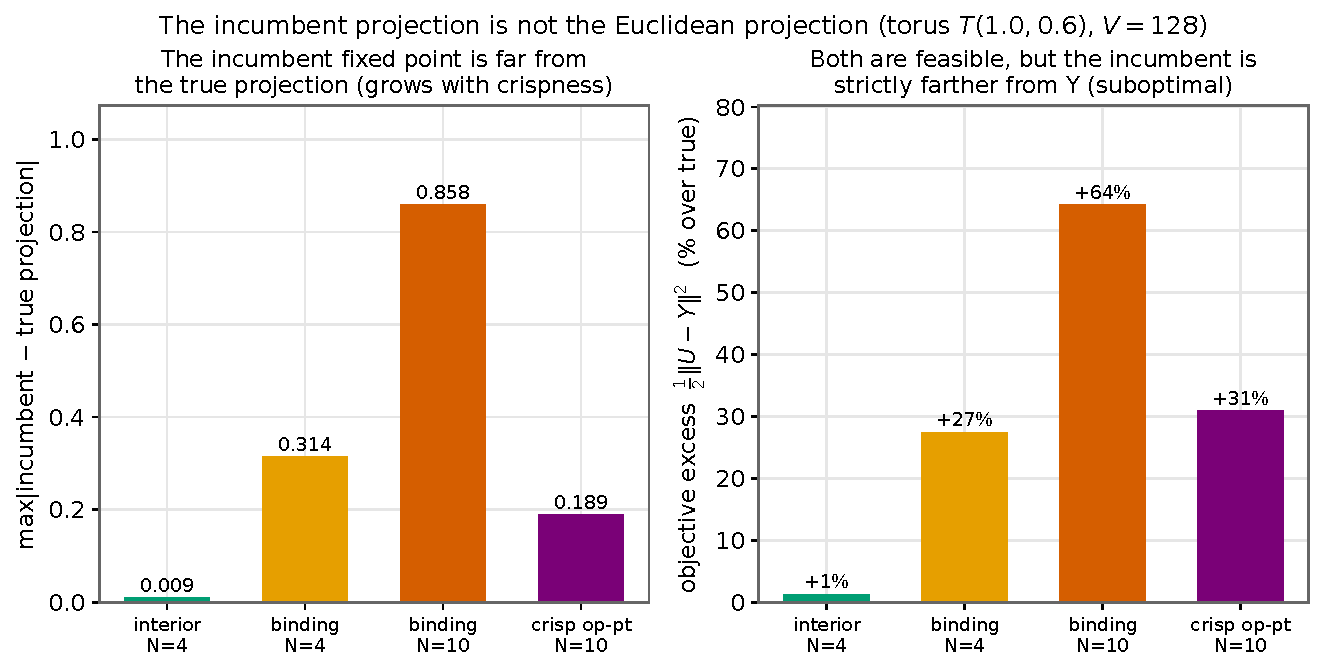
\includegraphics[width=\linewidth]{fig_projection_gap}
\caption{\emph{Left:} \(\max|\text{incumbent}-\text{true projection}|\) across regimes --- small
when the box is inactive (interior), large in the crisp/binding regime that is Phase~1's actual
operating point. \emph{Right:} the incumbent's objective \(\tfrac12\|U-Y\|^2\) excess over the
true minimum --- both points are feasible, but the incumbent is strictly farther from \(Y\), so
it is not the nearest feasible point.}
\label{fig:gap}
\end{figure}

\subsection{A solver-free certificate: the incumbent fails the dual-span test}
\label{sec:kkt}
The true projection's residual \(U-Y\) lies exactly in the span of the constraint duals (KKT
stationarity, Fig.~\ref{fig:kkt} left): the Dykstra reference satisfies it to \(\sim\!10^{-15}\)
in every regime. The incumbent's residual is \(0.01\)--\(1.16\) --- \(13\)--\(15\) orders of
magnitude larger --- so \(U_{\text{incumbent}}-Y\) is \emph{not} a combination of the row and
area dual directions, i.e.\ it is not the projection of \(Y\). This certificate needs no external
solver and is the cleanest single discriminator.

\subsection{Mechanism: it is the multiplicative row renormalization}
\label{sec:mechanism}
Why does the incumbent miss the projection even when the box is inactive? Its steps~1--9 are a
\emph{genuine} Euclidean affine projection onto \(\{\text{row}{=}1,\ \text{area}{=}d\}\) (verified
term-for-term against the \code{C} matrix at \code{projection.py:65-68}). But it first
\emph{multiplicatively} renormalizes each row (\(\div\) row sum, \code{projection.py:54-57}), and
its steps~10--12 (clip, then multiplicative row-renorm and column-rescale) are likewise not
Euclidean projections. The net effect is exact (Fig.~\ref{fig:kkt} right): the incumbent's
interior output equals the affine projection of the \emph{row-normalized} input,
\(|\,U_{\text{incumbent}} - P_{\text{aff}}(\text{rownorm}\,Y)\,| = 5.95{\times}10^{-12}\), versus
\(7.0{\times}10^{-3}\) against the affine projection of the raw \(Y\). It solves a nearby but
\emph{different} problem.

\begin{figure}[H]
\centering
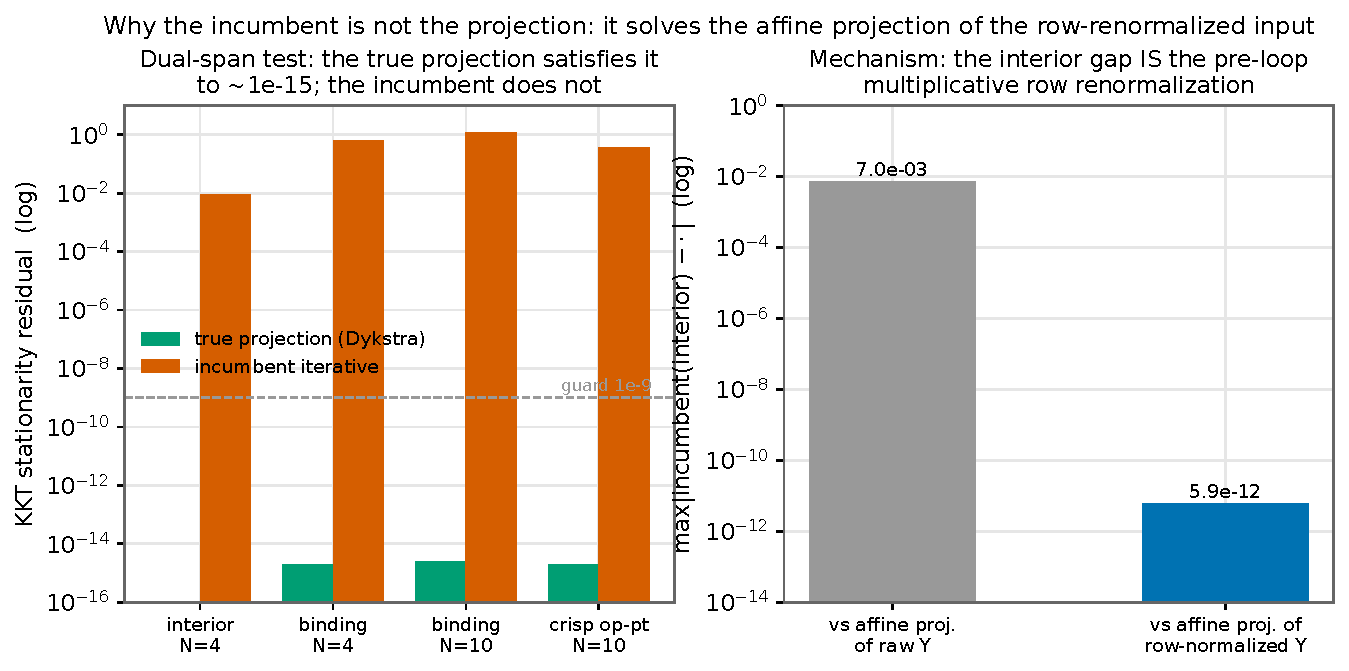
\includegraphics[width=\linewidth]{fig_kkt_certificate}
\caption{\emph{Left:} KKT stationarity residual (log) --- the true projection (green) passes to
\(\sim\!10^{-15}\); the incumbent (vermilion) fails by \(13\)--\(15\) orders across every regime.
\emph{Right:} the interior gap is entirely the pre-loop multiplicative row renormalization --- the
incumbent matches the affine projection of the row-normalized input to \(6{\times}10^{-12}\)
(blue), not the projection of the raw input (\(7{\times}10^{-3}\), grey).}
\label{fig:kkt}
\end{figure}

\subsection{Idempotency and the noise floor}
\label{sec:idem}
Re-projecting an \emph{exactly} feasible point barely moves it (\(3.5{\times}10^{-11}\); any
exactly feasible point is a fixed point of the map). But the PGD-level operation --- clip to
\([10^{-8},1{-}10^{-8}]\) \emph{then} project, which the optimizer runs every step --- moves an
already-feasible point by \(6.4{\times}10^{-8}\). That is the per-step noise floor that a true,
idempotent projection eliminates (the pre-clip becomes unnecessary once the projection returns
exact feasible entries, including hard \(0\)s).

\subsection{Implications, and an independent cross-check}
\label{sec:implications}
The core measurement was \textbf{independently reproduced} on 2026-07-19 by an adversarial review
using three algorithmically-unrelated exact references (closed-form affine projection, Dykstra,
and dual L-BFGS with an exact simplex oracle), agreeing pairwise to \(\leq 4{\times}10^{-9}\) and
cross-checked against \code{scipy} \code{trust-constr}; it found the gap reaches \(\sim\!0.9\) on
harsher inputs, confirming and extending Table~\ref{tab:gap}.

Two consequences for the replacement plan
(\codefile{docs/plans/PHASE1\_DUAL\_NEWTON\_PROJECTION\_PLAN.md}):
\begin{enumerate}[leftmargin=1.6em]
\item \textbf{The validation target is the true QP, not the incumbent.} A correct exact projection
  \emph{must} differ from \code{orthogonal\_projection\_iterative} by the amounts in
  Table~\ref{tab:gap}; ``match the incumbent to \(10^{-8}\)'' is unachievable and wrong. Validate
  against Dykstra + the KKT conditions instead.
\item \textbf{The replacement is a correctness upgrade, not a drop-in.} It changes the per-step
  projection (hence the PGD trajectory): exact, idempotent, and free of the
  \(6.4{\times}10^{-8}\) noise floor. Keep the incumbent byte-identical as the default; validate
  the new path end-to-end for partition \emph{validity}.
\end{enumerate}

\textbf{Partial (prototype) findings} from the same review, on a not-yet-implemented dual solver,
recorded here because they shaped the plan (they are measurements on prototypes, not committed
code): (i) the full LS-fit KKT certificate --- which also fits the active-set sign conditions ---
false-negatives (\(\approx 0.13\)) on the \emph{true} projection when a row is fully saturated
(one-hot, no inactive entry to pin \(\alpha_i\)); the plan's certificate must use the solver's own
duals. (ii) The area-constraint Jacobian of the dual is \emph{structurally} singular (\(J\cdot
\mathbf 1 = 0\)) and an empty cell makes an \(\varepsilon\)-ridge Newton step explode
(\(\sim\!10^{10}\)); the plan therefore adopts L-BFGS on the concave dual (robust to this) with a
gauge-fixed Newton polish. (iii) The pre-clip is not a no-op: \(\max|P(Y)-P(\text{clip}\,Y)|\)
reaches \(0.47\) on realistic inputs, so it is removed on the new path. These are documented in the
plan; this report's \emph{measured} claim is confined to \S\ref{sec:gap}--\S\ref{sec:idem}.

% =====================================================================
\section{Conclusion}
% =====================================================================
The Phase~1 constraint projection \code{orthogonal\_projection\_iterative}, documented and
profiled as \emph{the} Euclidean projection, does not compute it. It returns a feasible but
objective-suboptimal, path-dependent point --- exactly the affine projection of the
multiplicatively row-normalized input --- differing from the true nearest feasible point by up to
\(0.86\) (\(+64\%\) objective) in the crisp regime Phase~1 actually operates in, and failing the
KKT stationarity test the true projection passes to \(10^{-15}\). It is also only weakly
idempotent: the PGD clip-then-project step carries a \(\sim\!6{\times}10^{-8}\) per-iteration noise
floor. This is the evidence base for
\codefile{docs/plans/PHASE1\_DUAL\_NEWTON\_PROJECTION\_PLAN.md}: replacing the incumbent with an
\emph{exact} projection (via the concave dual) is a correctness upgrade as much as a speedup, and
must be validated against the true QP --- not against the incumbent it corrects.

% =====================================================================
\section*{Summary table}
% =====================================================================
\begin{center}\small
\begin{tabular}{@{}lll@{}}
\toprule
Quantity & Measured value & Source \\
\midrule
Metric of \eqref{eq:qp} & Euclidean (not \(v\)-weighted) & \code{projection.py:106}; \S\ref{sec:mechanism} \\
Max \(|\)incumbent\(-\)true\(|\) (crisp / binding) & \(0.19\) / up to \(0.86\) & Table~\ref{tab:gap}, \codefile{make\_figures.py} \\
Objective excess (binding \(N{=}10\)) & \(+64\%\) & Table~\ref{tab:gap} \\
KKT residual: true / incumbent & \(10^{-15}\) / \(0.01\)--\(1.16\) & Fig.~\ref{fig:kkt}; \code{stationarity\_residual} \\
Interior gap mechanism & \(P_{\text{aff}}(\text{rownorm}\,Y)\), resid \(6{\times}10^{-12}\) & \S\ref{sec:mechanism} \\
Idempotency: bare / clip-then-project & \(3.5{\times}10^{-11}\) / \(6.4{\times}10^{-8}\) & \S\ref{sec:idem} \\
\bottomrule
\end{tabular}
\end{center}

\end{document}
